\documentclass[tikz,border=10pt]{standalone}
\usepackage{tikz}
\usetikzlibrary{positioning, calc, arrows.meta}

\begin{document}

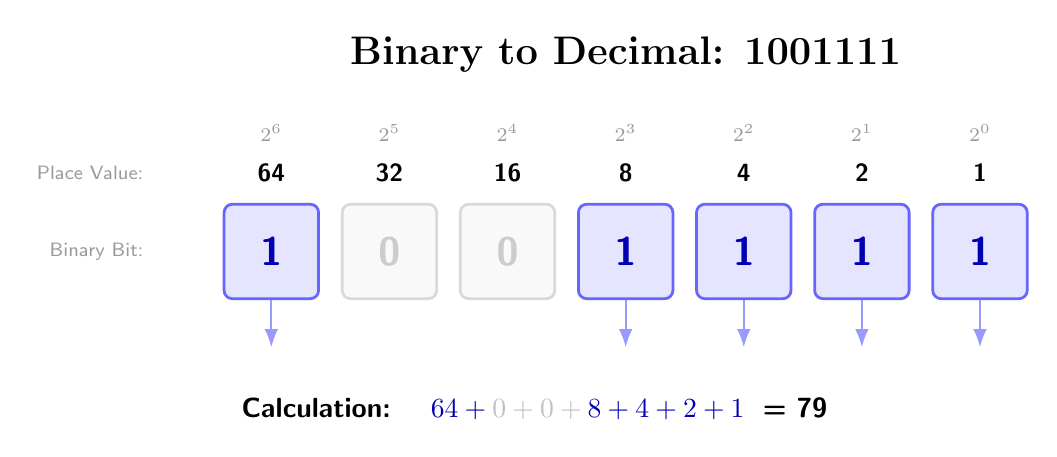
\begin{tikzpicture}[
    % Styling
    base font/.style={font=\sffamily},
    bit box/.style={
        draw, 
        minimum size=1.2cm, 
        rounded corners=3pt, 
        font=\sffamily\Large\bfseries,
        line width=1pt
    },
    % Style for '1' (Active)
    bit on/.style={
        bit box,
        fill=blue!10,
        draw=blue!60,
        text=blue!70!black
    },
    % Style for '0' (Inactive)
    bit off/.style={
        bit box,
        fill=gray!5,
        draw=gray!30,
        text=gray!40
    },
    label text/.style={
        font=\sffamily\scriptsize, 
        color=gray!80
    },
    value text/.style={
        font=\sffamily\small\bfseries
    },
    arrow style/.style={
        ->, 
        >={Latex}, 
        color=blue!40, 
        thick
    }
]

% --- Title ---
\node[base font, font=\Large\bfseries] at (4.5, 3) {Binary to Decimal: 1001111};

% --- The Loop ---
% We iterate through the bits. 
% Format: Power / Bit Value / Column Index
\foreach \power/\bit/\col in {6/1/0, 5/0/1, 4/0/2, 3/1/3, 2/1/4, 1/1/5, 0/1/6} {
    
    % Calculate X coordinate based on column index
    \pgfmathsetmacro{\xCoord}{\col * 1.5}
    
    % Calculate the Decimal Place Value (2^power)
    \pgfmathsetmacro{\placeVal}{int(2^\power)}

    % 1. Draw the Power Label (e.g., 2^6)
    \node[label text] at (\xCoord, 2) {$2^{\power}$};

    % 2. Draw the Decimal Value Label (e.g., 64)
    \node[value text] (val-\col) at (\xCoord, 1.5) {\placeVal};

    % 3. Draw the Bit Box (0 or 1)
    \ifnum\bit=1
        % If bit is 1: Use 'bit on' style
        \node[bit on] (box-\col) at (\xCoord, 0.5) {\bit};
        % Draw arrow pointing down to the math
        \draw[arrow style] (box-\col.south) -- ++(0, -0.6);
        % Add the value to the math string (visual only logic below)
    \else
        % If bit is 0: Use 'bit off' style
        \node[bit off] (box-\col) at (\xCoord, 0.5) {\bit};
    \fi
}

% --- The Calculation Row ---
% We manually construct the equation node to ensure perfect formatting
\node[base font, right, anchor=west] at (-0.5, -1.5) {
    \textbf{Calculation:} \quad
    $\color{blue!70!black}64 + \color{gray!50}0 + \color{gray!50}0 + \color{blue!70!black}8 + \color{blue!70!black}4 + \color{blue!70!black}2 + \color{blue!70!black}1$
    \space \textbf{= 79}
};

% --- Annotations ---
\node[label text, anchor=east] at (-1.5, 1.5) {Place Value:};
\node[label text, anchor=east] at (-1.5, 0.5) {Binary Bit:};

\end{tikzpicture}

\end{document}